\chapter{Theoretical Background}
\label{ch:02_Theoretical_Background}
\section{Single Pellet String Reactors}
The concept of a reactor, in which pellets are packed into tubes of only slightly larger diameter, emerged in the 1960s and was named as single pellet string reactor by Scott et al. \cite{Scott1974}. Therein, its resemblance to conventional packed beds with regards to flow behaviour was written in detail. The ease-of-use and convenience of SPSRs in a laboratory-scale for obtaining average diffusion coefficients across an array of temperatures and pressures with large porous particles was also highlighted.

In the chemical industry, the development, production and optimisation of new and existing heterogeneous catalysts plays a pivotal role. Performance evaluation of commercial catalysts is commonly accomplished at industrial process conditions, which requires the use of huge and expensive reactors with considerable gas flow rates, and with it, comes with the endangerment of engineers or technicians working on the reactor \cite{Heinemann1994}.

Thus, the general consensus would be to preferably achieve performance testing of catalysts at a much smaller scale. However, a multitude of problems such as axial convective and molecular diffusion, presents itself when attempting to downscale fixed-bed reactors, as presented by Sie \cite{Sie1996}. Sie also cited the effectiveness of so-called $nanoflow\:reactors$, which were essentially reactors below the scale of microreactors, in the testing of industrial catalysts. This points towards the applicability of SPSRs.

Ultimately, the struggle is in finding a small reactor that has the capability to house industrial-sized catalysts and demonstrates hydrodynamics which are sufficiently close to optimal plug flow. As such, SPSRs may just fit the bill. The underlying principle of optimal plug-flow reactors is that lateral mixing is sufficient without any mixing in the longitudinal direction \cite{San1989}.



The idea of adding small inert particles to the catalytic bed which is present in this simulative work was put forward by both Sie \cite{Sie1996} and Gierman \cite{Gierman1988}. In an attempt to improve the isothermal properties of catalytic fixed beds, Gierman \cite{Gierman1988} added small inert particles to the catalytic bed which reduces wall effects and improves plug flow. While operating in trickle-flow, Sie \cite{Sie1996} stated the need for the addition of fine particles in small beds of large industrial catalyst particles to ensure near plug flow hydrodynamics.
%Hence, it is practice to use shorter or narrower catalyst beds with smaller catalyst particles in an attempt to mimic commercial process conditions, albeit in a much smaller scale. However, is it of great importance that the 
%The need for performance evaluation of commericial catalysts at industrial process conditions albeit in a much smaller scale \cite{Heinemann1994} makes SPSRs the ideal candidate in terms of economical and safety reasons.
%- There needs to be further proving/ understanding of SPSRs through experimental and simulative works so that they can be applied in the chemical industry for the advantages/benefits that come along with using it.
%- talk about history/development of SPSRs, as well as pressure drops correlations,
\section{Numerical Simulation with CFD}
Numerical simulation is a powerful, time-saving tool in which virtual models can be used to estimate the changes in parameters (such as pressure, temperature) across a stipulated physical and simulative time-frame. It is a form of simulation by which calculation is done on a computer with the user's choice of simulative program that implements a mathematical model for a physical system. Commonly used by data scientists and researchers, it is a powerful tool which leverage on the processing and computational power of computers to solve often complex non-linear systems of equations that will otherwise takes months to solve by conventional pen-and-paper methods. With the advent of numerical simulation, engineers and scientists alike would no longer have to go through various cycles of building and destroying physical prototypes of models to achieve the desired final products for their clients.

Computational Fluid Dynamics (CFD) software such as OpenFOAM\textsuperscript{\textregistered} utilises a modelling technique that breaks down governing equations (continuity, momentum and energy) of fluid flow into simpler forms that can be solved via numerical techniques \cite{Blocken2004}. CFD then uses models to approximate some components of the flow. Since there are no universal rules or guidelines on the appropriateness of models to use, the burden is on the user to select the right model tailored to solve the desired problem on hand. Although computer modelling can be used to predict results, validation with experimental data is always necessary to verify the accuracy of the solution.
%As in most nonlinear systems, computational simulations are required to test the actions of structures whose mathematical models are too complicated to provide practical solutions.
%https://www.openfoam.com/documentation/user-guide/standard-solvers.php
%https://www.openfoam.com/documentation/guides/latest/doc/guide-applications-solvers-incompressible-simpleFoam.html
%https://www.bizjournals.com/phoenix/blog/techflash/2016/04/what-is-numerical-simulation-and-why-should-i.html
%https://www.nature.com/subjects/numerical-simulations
\subsection{OpenFOAM as a CFD Program}
OpenFOAM\textsuperscript{\textregistered} is an acronym which stands for $Open\:Source\:Field\:Operation\:and\:Manipulation$. As the name implies, the program is open source and free in nature, meaning that its source code and libraries are available for users to edit and improve upon, thus thriving on the spirit of collaborative work from users on the Internet \cite{Chen2014}. This signifies that users no longer have to spend long periods of time writing CFD codes or purchase (often) expensive commercial software. Through the solving of mathematical models, an approximation as to what happens in a single volume element (grid) in the simulative environment can be achieved, thus painting a picture as to what would be observed in reality.

The workflow of an OpenFOAM\textsuperscript{\textregistered} simulation can be broken down into 3 main parts which are described briefly below:
\begin{enumerate}
	\item $Preprocessing$
	\\$Mesh\;generation$ is performed during this phase. In simpler cases, the use of the $blockMesh$ utility is sufficient. In the case of more complicated geometries as in this study, a combination of $blockMesh$, $snappyHexMesh$ and third-party programs such as Blender\texttrademark\:can be used in the generation of the confining cylinder and the packing arrangement.
	\item $Solving$
	\\As opposed to confining its users to a universal solver as typically seen in commercial CFD programs, OpenFOAM\textsuperscript{\textregistered} does not have a generic solver applicable to all cases. Rather, the solvers present in OpenFOAM\textsuperscript{\textregistered} are tailored to specific physics in the broad categories of different flow types and continuum mechanics that are, but not limited to: incompressible flow, compressible flow, multiphase flow, heat transfer and buoyancy-driven flows, particle-tracking flows and combustion \cite{Chen2014}. In this case, the \emph{simpleFoam} solver is used.
%101 different types of standard solvers
	\item $Postprocessing$
	\\To produce graphical output of the simulated numerical values, OpenFOAM\textsuperscript{\textregistered} uses an open-source, multiplatform data analysis and visualization application known as $ParaView$. In $ParaView$, users can utilise a plethora of postprocessing tools to visualise the change in parameters in the model throughout the iterative steps or physical time depending on the type of solver specified under the $solving$ step.
\end{enumerate}
% talk about friction factor trends, pressure drop, i.e. importance of pressure drop
%The SIMPLE pressure-velocity algorithms are tied to both the momentum and continuity equation are depicted in Eqns. \ref{momentum_eqn_openfoamwiki} and \ref{continuity_eqn}
%\begin{equation}\label{momentum_eqn_openfoamuserguide}
%\frac{\partial}{\partial t}(u) + \nabla\cdot(u\otimes u) = -\Delta p
%\end{equation}
%\begin{equation} \label{continuity_eqn_openfoamuserguide}
%\nabla\cdot u = 0
%\end{equation}
%\begin{equation} \label{momentum_eqn_josefnagy}
%\nabla\cdot(uu)=-\frac{1}{\rho}\nabla p+\nabla\cdot\nu[2S]+F_t
%\end{equation}
%\begin{equation}\label{pressure_josefnagy}
%p = \frac{1}{\rho} \overline{p}
%\end{equation}
%https://openfoamwiki.net/index.php/SimpleFoam
\subsection{Turbulence Modelling}
Turbulence modelling is a technique to contrive a number of partial differential equations for turbulent-flow calculation, founded from approximation of the Navier-Stokes equation.

OpenFOAM\textsuperscript{\textregistered} offers a wide range of turbulence simulation methods and models via its \emph{TurbulenceModels} library. The library supports: models for constant and variable density (incompressible and compressible flows), inclusion of buoyancy terms (models for single and multiphase flows) and the configuration of sources and constraints in case input files. There are 3 main types of turbulence modelling present in OpenFOAM\textsuperscript{\textregistered}, namely Reynolds-Averaged Simulation (RAS) or Reynolds-averaged Navier-Stokes (RANS), Direct Numerical Simulation (DNS), and Large Eddy Simulation (LES).

More often than not, turbulent flows are difficult to simulate owing to their randomness. The amount of information obtained from a simulation is directly proportional to the computational cost. Whilst LES and DNS offers a high degree of details, it requires prohibitively large simulation times.
Mathematical expression and diffusion term of viscous stresses differ between Newtonian fluids and non-Newtonian fluids. Many turbulence models treat the effect of turbulence as an augmentation of mixing or diffusion. The modelled expression however, varies based on the selected turbulence models (linear eddy-viscosity, non-linear eddy viscosity, Reynolds-stress transport models under RANS).

In RANS, the Reynolds decomposition of the flow variables is accomplished by first separating the flow variables into mean and fluctuating parts \cite{Alfonsi2009}. Following which the Reynolds-decomposed variables are inserted into the Navier-Stokes equations. The averaging of the equations yields the Reynolds-stress tensor term, which has to be modelled for the RANS equations to be solved. Thus, additional (closure) equations are required to solve the system. These equations are derived from higher-order moments of the averaged Navier-Stokes equation with additional assumptions based on the knowledge of the properties of turbulent flow, resulting in a modified set of equations that is less-computationally intensive to solve \cite{Pisarenco2011}. An outline of the aforementioned steps is listed in the section below.
\subsubsection{Reynolds Decomposition and Averaging} The following equations for the decomposition of flow variables in RANS are obtained from Alfonsi et al. \cite{Alfonsi2009}. The flow of a viscous incompressible fluid having constant properties is given by the Navier-Stokes equations:
\begin{equation}\label{Navier_Stokes_Alfonsi_1}
	\frac{\partial u_i}{\partial t} + \frac{\partial}{\partial x_j}(u_iu_j) = -\frac{\partial p}{\partial x_i} + \nu\frac{\partial^2 u_i}{\partial x_j \partial x_j}
\end{equation}
\begin{equation}\label{Navier_Stokes_Alfonsi_2}
	\frac{\partial u_i}{\partial x_i} = 0
\end{equation}
where $u_i$ is the fluid velocity, $p$ being the pressure divided by the density $\rho$, $\nu$ is the fluid kinematic viscosity. Body forces do not appear explicitly, and the convective term of Equation \eqref{Navier_Stokes_Alfonsi_1} is being expressed in conservative form. The Reynolds decomposition in RANS proceeds via the decomposition of the dependent variables of Equations \eqref{Navier_Stokes_Alfonsi_1} and \eqref{Navier_Stokes_Alfonsi_2} into mean and fluctuating parts:
\begin{equation} \label{u_i_Alfonsi}
u_i = \overline{u}_i + u_i^\prime,\;p = \overline{p} + p\prime
\end{equation}
under the assumption as proposed by Tennekes et al. \cite{Tennekes1972}, that the following properties of the average operator hold:
\begin{equation} \label{average_operator_Alfonsi_1}
	\overline{\phi\prime} = \overline{\psi\prime} = 0,
\qquad
	\overline{\phi\psi} = \overline{\phi}\overline{\psi} + \overline{\phi\prime\psi\prime},
\qquad
	\overline{\overline{\phi}\phi\prime} = \overline{\overline{\psi}\psi\prime} = \overline{\overline{\phi}\psi\prime} = \overline{\overline{\psi}\phi\prime} = 0
\end{equation}
\begin{equation} 	\label{average_operator_Alfonsi_2}
	\overline{\phi^2} = \overline{\phi}^2 + \overline{\phi\prime^2},
	\qquad
	\frac{\overline{\partial\phi}}{\partial t} = \frac{\partial\overline{\phi}}{\partial t},
	\qquad
	\frac{\overline{\partial\phi}}{\partial x_i} = \frac{\partial\overline{\phi}}{\partial x_i}
\end{equation}
with $\phi$ and $\psi$ being a representative of two generic flow variables. The mean value of any generic variable ($\phi$) can be calculated, in a turbulent statistically steady state as a time average ($\overline{\phi}^T$) and in a turbulent spatially homogeneous flow as a volume average ($\overline{\phi}^V$). In a turbulent flow of a general nature the mean can be computed as an ensemble average:
\begin{equation}
	\overline{\phi}^E(\textbf{x},t) = \lim_{N \to \infty} \frac{1}{N}\sum\limits_{k=1}^N \phi^k(\textbf{x},t)
\end{equation}
in which N represents the number of repeated experiments. In a turbulent statistically steady state and in a turbulent spatially homogeneous flow:
\begin{equation}
\overline{\phi}^T = \overline{\phi}^E,\;\overline{\phi}^V = \overline{\phi}^E
\end{equation}
Via substitution of Eq. \ref{u_i_Alfonsi} into Eqs. \ref{Navier_Stokes_Alfonsi_1} and \ref{Navier_Stokes_Alfonsi_2}, taking an ensemble average and enforcing properties \ref{average_operator_Alfonsi_1} and \ref{average_operator_Alfonsi_2}, a system of partial differential equations that governs the mean-velocity and pressure fields of incompressible turbulent flow is obtained as:
\begin{equation} \label{systemofpartialdifferentialequations_Alfonsi}
	\frac{\partial \overline{u}_i}{\partial t} + \frac{\partial}{\partial x_j}(\overline{u_i u_j}) = -\frac{\partial\overline{p}}{\partial x_i} + \nu\frac{\partial^2 \overline{u}_i}{\partial x_j \partial x_j}
\end{equation}
\begin{equation}
	\frac{\partial\overline{u_i}}{\partial x_i} = 0
\end{equation}
Referencing the nonlinear term of eqs. \ref{systemofpartialdifferentialequations_Alfonsi}, one obtains:
\begin{equation}
	\overline{u_i u_j} =
	 \overline{(\overline{u}_i + u_i^\prime)(\overline{u}_j + u_j^\prime)} =
	  \overline{\overline{u}_i\overline{u}_j} + 
	  \overline{\overline{u}_i u_j^\prime} +
	   \overline{{u}_i^\prime\overline{u}_j} + 
		\overline{u_i^\prime u_j^\prime} =
		\overline{u}_i \overline{u}_j +
		\overline{u_i^\prime u_j^\prime}
\end{equation}
that gives:
\begin{equation}
	\frac{\partial\overline{u}_i}{\partial t} + \frac{\partial}{\partial x_j}(\overline{u}_i\overline{u}_j) = - \frac{\partial\overline{p}}{\partial x_i} + \nu\frac{\partial^2\overline{u}_i}{\partial x_j \partial x_j} - \frac{\partial}{\partial x_j} (\overline{u_i^\prime u_j^\prime})
\end{equation}
Thus, the RANS as projected by \cite{Hinze1975} is obtained:
\begin{equation} \label{obtainedRANS_Alfonsi_1}
	\frac{\partial\overline{u}_i}{\partial t} + \overline{u}_j \frac{\partial\overline{u}_i}{\partial x_j} = - \frac{\partial\overline{p}}{\partial x_i} + \nu\frac{\partial^2\overline{u}_i}{\partial x_j \partial x_j} - \frac{\partial\tau_{ij}}{\partial x_j}
\end{equation}
\begin{equation} \label{obtainedRANS_Alfonsi_2}
	\frac{\partial\overline{u}_i}{\partial x_i} = 0
\end{equation}
where the convective term of Eq. \ref{obtainedRANS_Alfonsi_1} is expressed in non-conservative form, and:
\begin{equation}
	\tau_{ij} = \overline{u_i^\prime u_j^\prime}
\end{equation}
gives the $Reynolds-stress\;Term$ ($Reynolds-stress\;Tensor$ divided by the density) which includes the effects of turbulent motions on the mean stresses.

The Reynolds-stress tensor is symmetric, and the diagonal components give the normal stresses, while the off-diagonal components are correlated to shear stresses. \ref{obtainedRANS_Alfonsi_1} and \ref{obtainedRANS_Alfonsi_2} are not a closed system for the calculation of the dependent variables, $\overline{u}_i$ and $\overline{p}$, in the context that the Reynolds-stress tensor includes six additional independent unknowns. The problem with the closure of the Reynolds-averaged Navier-Stokes equations consists mainly in the formulation of the Reynolds-stress tensor as a function of the mean-field and/or other variables.
Generally, turbulence models are designed to represent high-order moments of turbulence variability in lower-order moments. This can be done directly, as in the case of eddy viscosity models, or implicitly, as with the case of models based on the solution of additional partial differential equations.

In this study, RANS was considered to be the best turbulence model for the base case, as the increased computational load used for the depiction of eddies associated with the LES model would not be useful in obtaining an averaged pressure drop in a SPSR owing it's small confining diameter. It should be mentioned that the effectiveness of the RANS model requires careful monitoring of the $y+$ value, which is connected to the mesh refinement.
%https://caefn.com/tag/rans -> fumiya explanation of RANS
%CONFIRMED THAT RAS = RANS, Source -> https://cfd.direct/openfoam/features/turbulence-modelling/
%Reynolds-average simulation (RAS), also known as Reynolds-averaged Navier-Stokes (RANS): The governing equations are solved in ensemble-averaged form, including appropriate models for the effect of turbulence. See the list of RAS models for more information.
%RAS
%
%high Reynolds number: first cell height should be in the region of 30 < y+ < 200. Note that the upper limit is imposed by the location of the outer layer, which depends on the Reynolds number
%low Reynolds number: mesh required to resolve the viscous sub-layer, typically using 10-20 layers
%LES
%
%mesh required to resolve the viscous sub-layer
%requires high order schemes to adequately resolve the high-energy containing eddies
%preferably isotropic mesh
\subsection{$k-\omega$-SST model}
The $k-\omega$-SST model is a linear eddy viscosity model stemmed from RANS. The turbulence model used in this work is the $k-\omega$-SST model, which is an extension of the standard $k-\omega$ model widely popularised by Wilcox, D.C \cite{Wilcox1993a}. In the standard k-$\omega$ model, two additional transport equations with variables $k$ and $\omega$ are introduced as a description of turbulent kinetic energy and the scale of turbulence respectively. The model by Wilcox is sensitive to the freestream value of omega, $\omega_f$, thus leading to great deviations in the obtained simulative friction factor if an erroneous prediction of $\omega_f$ is made and hence was not used in this study.
%unsure if \cite{Wilcox1988} truely is the original k-omega model proposed by \cite{Wilcox1993a}
%mentions about the blending function of the omega
\subsubsection{SST Model Formulation}
The complete formulation of the SST model taken from Menter et al.  \cite{Menter2003} is outlined and modifications to the original k-$\omega$ model are highlighted:
\begin{equation}
	\frac{\partial(\rho k)}{\partial t} + \frac{\partial(\rho U_i k)}{\partial x_i} = \tilde{P}_k - \beta^\ast\rho k \omega + \frac{\partial}{\partial x_i} \Big[(\mu+\sigma_k\mu_t)\frac{\partial k}{\partial x_i}\Big]
\end{equation}
\begin{equation}
	\frac{\partial(\rho\omega)}{\partial t} + \frac{\partial(\rho U_i \omega)}{\partial x_i} = \alpha\rho S^2 - \beta\rho\omega^2 + \frac{\partial}{\partial x_i} \Big[(\mu + \sigma_\omega \mu_t)\frac{\partial\omega}{\partial x_i}\Big] + 2 (1-F_1)\rho\sigma_{\omega 2} \frac{1}{\omega} \frac{\partial k}{\partial x_i} \frac{\partial\omega}{\partial x_i}
\end{equation}
In which the blending function $F_1$ is defined by:
\begin{equation}
	F_1 = \tanh\Bigg\{\bigg\{min\Big[max\Big(\frac{\sqrt{k}}{\beta^\ast\omega y},\frac{500\nu}{y^2\omega}\Big),\frac{4\rho\sigma_{\omega 2}k}{CD_{k\omega}y^2}}\Big]\bigg\}^4\Bigg\}
\end{equation}
with $CD_{k\omega} = max\Big(2\rho\sigma_{\omega 2}\frac{1}{\omega}\frac{\partial k}{\partial x_i}\frac{\partial\omega}{\partial x_i}, 10^{-10}\Big)$ and $y$ is the distance to the nearest wall.

$F_1$ becomes zero away from the surface ($k$-$\epsilon$ model), and switches to one inside the boundary layer ($k$-$\omega$ model).
The turbulent eddy viscosity is defined as:
\begin{equation}\label{turbulenteddyviscosity_menter}
	\nu_t = \frac{a_1 k}{max(a_1\omega,S F_2)}
\end{equation}
where $S$ is the invariant measure of the strain rate and $F_2$ is a second blending function defined as:
\begin{equation}
	F_2 = \tanh\bigg[\Big[max\big(\frac{2\sqrt{k}}{\beta^\ast\omega y},\frac{500\nu}{y^2\omega}\big)\Big]^2\bigg]
\end{equation}
A production limiter is used in the SST model for the prevention of build-up of turbulence in stagnant regions:
\begin{equation}
	P_k = \mu_t\frac{\partial U_i}{\partial x_j}\bigg(\frac{\partial U_i}{\partial x_j} + \frac{\partial U_j}{\partial x_i}\bigg) \rightarrow \tilde{P}_k = min \big(P_k,10\cdot\beta^\ast\rho k\omega\big)
\end{equation}
All constants are calculated by blending the corresponding constants from the $k-\epsilon$ and $k-\omega$ model via $\alpha = \alpha_1F + \alpha_2(1-F)$ etc. The constants for this model are: $\beta^\ast = 0.09$, $\alpha_1$ = 5/9, $\beta_1$ = 3/40, $\sigma_{k1}$ = 0.85, $\sigma_{\omega1}$ = 0.5, $\alpha_2$ = 0.44, $\beta_2$ = 0.0828, $\sigma_{k2}$ = 1, $\sigma_{\omega2}$ = 0.856.
The only modifications made from the original expression is the use of the strain rate, $S$, rather than the vorticity in Eq. \ref{turbulenteddyviscosity_menter}, and the use of factor 10 in the production limiter, as opposed to 20 as proposed by Menter et al. \cite{Menter1993,Menter1994}. Although less sensitive to the freestream values of $\omega$ as compared to the standard $k-\omega$ model, an educated prediction of $\omega$ must be done for the \emph{simpleFoam} solver to work with.

Despite its popularity as a turbulence model used for practical calculations \cite{Rodi1991}, the $k-\epsilon$-model is not used in this work as it does not handle surface boundaries well.

The $k-\omega$-SST model used in OpenFOAM\textsuperscript{\textregistered} is obtained from the 2003 model by Menter et. al. \cite{Menter2003}.

%https://cfd.spbstu.ru/agarbaruk/doc/2003_Menter,%20Kuntz,%20Langtry_Ten%20years%20of%20industrial%20experience%20with%20the%20SST%20turbulence%20model.pdf
%^ article explanating about the derivation of SST model as for [8], "a new near wall treatment was therefore developed [8], which automatically shifts from the standard low-Re formulation to wall functions, based on grid spacing of the near-wall cell.
\subsection{The law of the wall}
Due to large velocity gradients arising in the region near the wall, flow considered in the near-wall region is no longer turbulent. Thus, assumptions made while deriving the turbulence models are not applicable in this region.

The boundary layer velocity profile is subdivided into three regions through analytical equation derivations and experimental evidence fitting and is listed in order from increasing distance from the wall: the laminar sublayer, the buffer area, and the log-law zone \cite{Chen1998, Blocken2004}.

In the linear/laminar sublayer, the laminar law holds to which the dimensionless velocity is equals to the dimensionless wall coordinate (i.e. $u^+$ = $y^+$). In this region, the fluid is dominated by viscous effects hence negligible Reynolds shear stress is assumed. In the log-law zone, turbulence stress dominates the flow and the velocity profile vary very slowly with the logarithmic function along the distance. In this region, the logarithmic law is valid and is given by $u^+ = \ln(y^+)/\kappa+B$ where $\kappa$ represents the Karman constant, $\kappa$ = 0.41, and $B$ the integration constant with $B \approx 5.0-5.4$ \cite{Schlichting1960, White2006}. Laminar law is valid for $y^+ <5$ while logarithmic law is true for $y^+ > 30$ up to $y^+ = 500-1000$ \cite{Blocken2007}.

A visual representation of the aforementioned zones is depicted in Fig. \ref{fig:LawOfTheWall} \cite{Nezu2000}:
\newpage
\begin{figure}[ht]
	\centering
	\caption{Plot of the dimensionless velocity, $u^+$, against the dimensionless wall coordinate, $y+$, showing different zones of interest.}
	\label{fig:LawOfTheWall}
	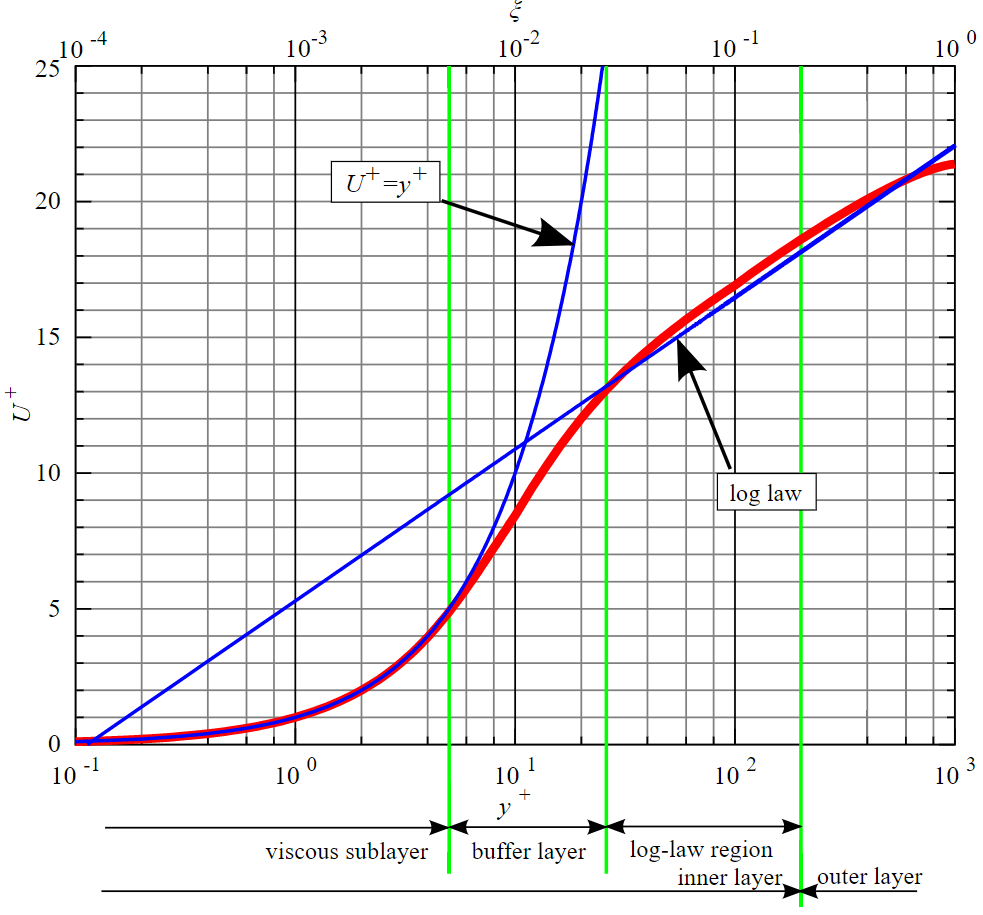
\includegraphics[width=0.5\linewidth]{Figures/LawOfTheWall.png}
\end{figure} 

Two general approaches are usually employed in CFD when modelling the flow in the near-wall region, Low-Reynolds-number (low-Re) modelling and Wall function theory.
In the Low-Re approach, the boundary layer is sufficiently fine meshed such that the first cell is placed entirely in the laminar sublayer of the boundary layer, with the height of the first cell corresponding to a value of $y+ \approx 1$ (although validity of laminar sublayer still holds true up till $y^+ < 5$) \cite{Blocken2004}, allowing the governing equations of fluid flow to be solved in all regions of the boundary layer.

In the second approach, the viscosity-affected inner region (with respect to the wall) which consists of the viscous sublayer and buffer layer is not resolved through fine mesh generation. Instead, the usage of semi-empirical wall functions are used to bridge the viscosity-affected region between the wall and the fully-turbulent region \cite{Pisarenco2011}. Wall functions are commonly used with coarser meshes in which the first cell is found at $y^+ > 30$. The use of wall functions avert the need for the modification of the turbulent models to account for the presence of the wall. This substantially saves computational resources in most high-Reynolds-number flows, because the near-wall region that is affected by viscosity, in which the solution variables change most rapidly, need not be resolved. As such, this approach is popular for near-wall treatment in industrial flow simulations because it is economical, robust, practical and reasonably accurate.

Having the height of the first cell land in the range of $5 < y^+ < 30$ puts it in the buffer region, which is situated between the laminar sublayer and the log-law region of the boundary layer. It is generally not advisable to have the first cell land in this region as it amounts to less accurate results obtained with either of the two methods listed above \cite{Salim2009}.

Simulations on the base case were ran with and without wall functions being applied to $k$, $\omega$ and the model turbulent viscosity, $\nu_t$. In RANS, only the mean velocity $\overline u$ is considered and the oscillating velocity term $u^\prime(t)$ is omitted thus leading to errors. Hence, the correct edition and inclusion of the model turbulent viscosity $\nu_t$ is paramount to account for the transport and dissipation of energy neglected from the removal of $u^\prime(t)$.

The effective viscosity, $\nu_{eff}$, in RANS as a function of the model turbulent viscosity and the physical viscosity thus given by: $\nu_{eff}$ = $\nu$ + $\nu_t$

Due to the fineness of the mesh associated in the original base case as generated by Fernengel et al. \cite{Fernengel2020}, an extremely low $y+$ value in the range of $y+ < 2$ was obtained with $k-\omega$-SST with RANS simulation which places the height of the first cell in the laminar sublayer (cf. Fig. \ref{fig:Slice_MeshFineness_zoomed1_CaseA}). A general rule of thumb when using wall functions is to obtain $y+$ values between 30 and 200 as this allows the first cell centre to be placed in the log-law region to ensure accuracy of the results.

\begin{figure} [h]
	\centering
	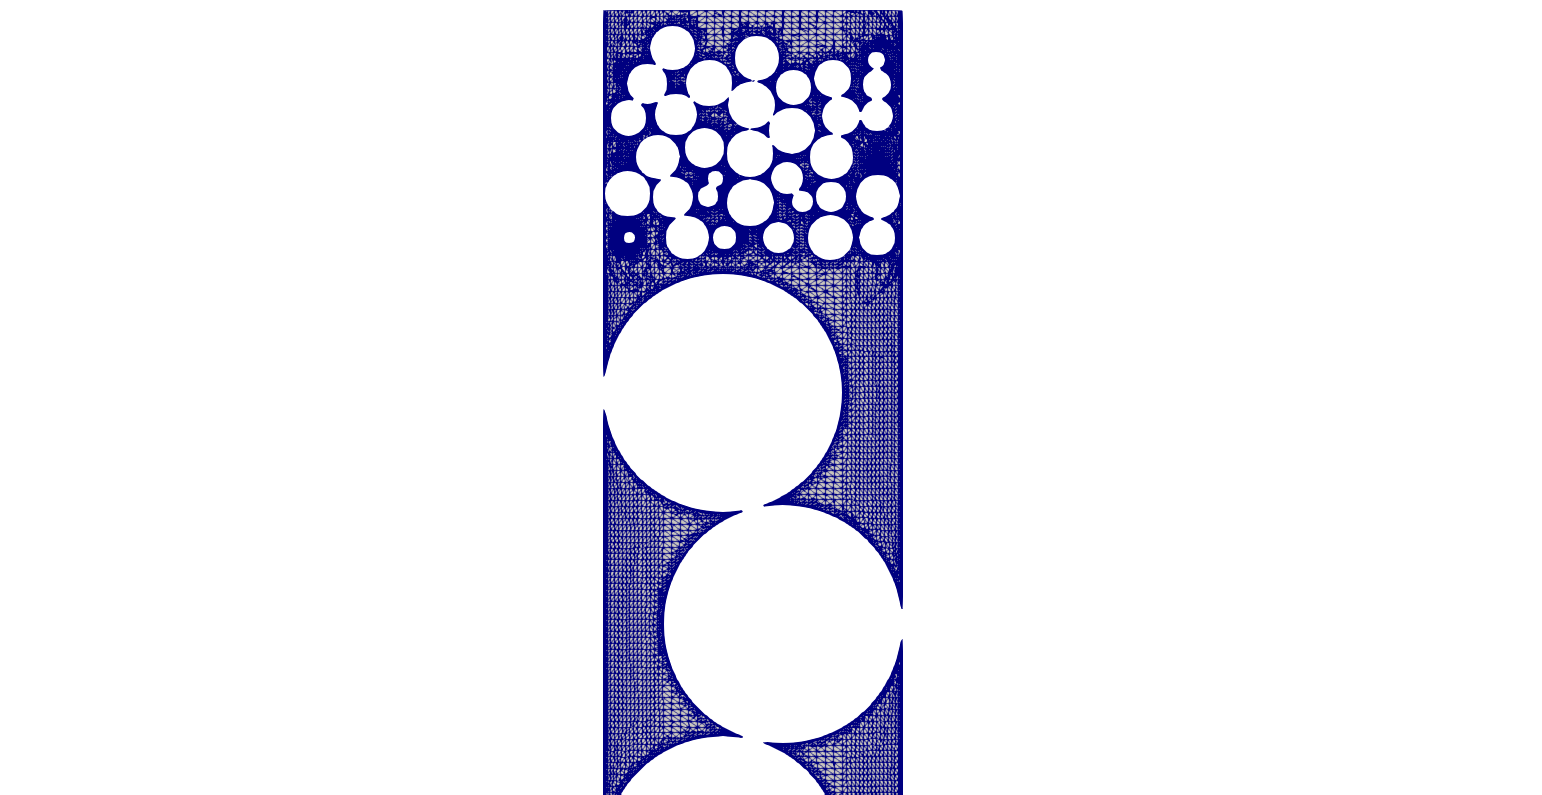
\includegraphics[width=0.5\linewidth]{Figures/visualisation/caseA/Slice_MeshFineness_zoomed1_CaseA.png}
	\caption{Slice of Base Case Showing Mesh Resolution.}
	\label{fig:Slice_MeshFineness_zoomed1_CaseA}
\end{figure}
The $\omega$ wall function is a special wall function that is able to switch between viscous and log-law region \cite{Liu2016}. Furthermore, the $k-\omega$-SST by Menter has the ability to automatically shift from the standard low-Re formulation to wall function, based on grid spacing of the near-wall cell. Hence, using the turbulence model based on $\omega$ (such as the $k-\omega$-SST model) should technically yield accurate results.

However, the obtained simulative results with wall functions yielded a pressure drop that gave a less-than-expected friction factor that does not correspond to friction factor values shown in Fig. \ref{fig:ComparisonAcrossSPSRVariations}. As such, it can be inferred that the $k-\omega$-SST model is best utilized without wall functions should a fine mesh be used as with this base case.
%-y+ values, what they are, how does it play a role in the simulation, and why ultimately wall functions were not used in the simulation
 %In the OpenFOAM omegaWallFunction is a special wall function which can switch
%between viscous and logarithmic region according to the position of y
%+. In the intersection of the
%viscous sublayer and log-law region value is calculated through blending the viscous and log-law
%sublayer value. liu2016
